\documentclass[10pt,a4paper, margin=1in]{article}
\usepackage{fullpage}
\usepackage{amsfonts, amsmath, pifont}
\usepackage{amsthm}
\usepackage{graphicx}
\usepackage{float}

\usepackage{listings}

\usepackage{tkz-euclide}
\usepackage{tikz}
\usepackage{pgfplots}
\pgfplotsset{compat=1.13}

\usepackage{geometry}
 \geometry{
 a4paper,
 total={210mm,297mm},
 left=10mm,
 right=10mm,
 top=10mm,
 bottom=10mm,
 }
 % Write both of your names here. Fill exxxxxxx with your ceng mail address.
 \author{
  İşleyici, Osman Taylan\\
  \texttt{e2448496@ceng.metu.edu.tr}
  \and
  LastName2, FirstName2\\
  \texttt{exxxxxxx@ceng.metu.edu.tr}
}

\title{CENG 384 - Signals and Systems for Computer Engineers \\
Spring 2023 \\
Homework 1}
\begin{document}
\maketitle



\noindent\rule{19cm}{1.2pt}

\begin{enumerate}

    \item %write the solution of q1
          \begin{enumerate}
              % Write your solutions in the following items.
              \item %write the solution of q1a
              \item %write the solution of q1b
              \item %write the solution of q1c
              \item %write the solution of q1d
          \end{enumerate}

    \item ~\\
          \begin{figure}[H]
              \centering
              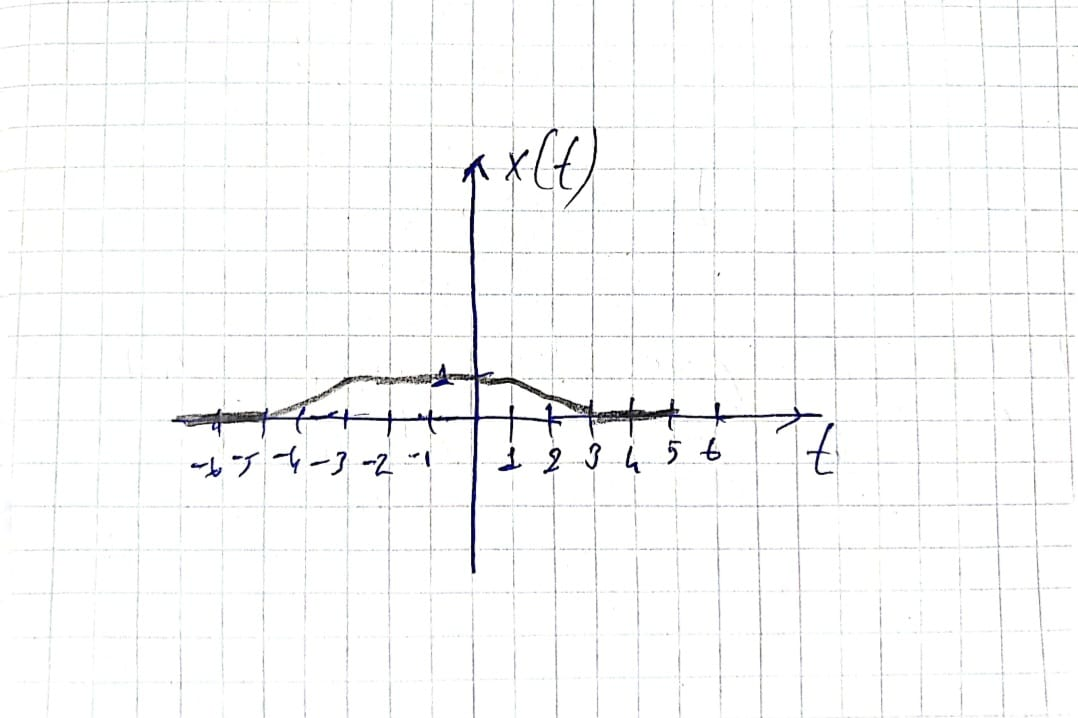
\includegraphics[scale=0.25]{handwritten_signal.jpeg}
              \caption{Signal $x(\frac{1}{2}t+1)$}
          \end{figure}

    \item %write the solution of q3
          \begin{enumerate}
              % Write your solutions in the following items.
              \item %write the solution of q3a
              \item %write the solution of q3b
          \end{enumerate}

    \item %q4
          \begin{enumerate}
              \item The signal is periodic and its fundamental period is $\frac{2 \pi}{3}$ since the fundamental
                    period of signal $k*cos(at+b)$ is determined by $\frac{2 \pi}{a}$.
              \item The fundamental period of discrete signal $mcos[an+b]$ is the smallest integer $\frac{2\pi k }{a}$ where k is any integer. Here the period of cosine part is 20, and the period of the sine part is 20 too. So the period of signal itself is least common multiple of these two periods, 20. The signal is periodic.
              \item Since there isn't any integer k which makes $\frac{2\pi k}{7}$ an integer. The signal is not periodic.
          \end{enumerate}

    \item %write the solution of q5
          \begin{enumerate}
              % Write your solutions in the following items.
              \item %write the solution of q5a
              \item %write the solution of q5b
          \end{enumerate}

    \item %write the solution of q6
          \begin{enumerate}
              % Write your solutions in the following items.
              \item
                    \begin{itemize}
                        \item It has a memory since output depends on input $x(2t+3)$.
                        \item It's not stable. We can prove this by counterexample, if $x(t) = 1$, $y(t) = t$ which is an unbounded output. So bounded inputs ($1$) yields unbounded outputs.
                        \item It's not causal since the output depends on inputs greater than t if $t>-3$.
                        \item It's linear since for two input signals $x_1$ and $x_2$ and their corresponding outputs $y_1$ and $y_2$; $ay_1(t)+ by_2(t) = atx_1(2t+3) + btx_2(2t+3)$ is equal to $y_3(t) = tx_3(2t+3)$ where $x_3$ is $ax_1+b_x2$.
                        \item It's invertible since we can write a system $w(t) = \frac{2y(\frac{t-3}{2})}{t-3}$ whose output for the signal $y(t)$ is $x(t)$.
                        \item The system is time varying because of two reasons, there is a time scaling on input $(2t+3)$, and there is also a time multiplier on signal. Both these reasons are enough for time variance.
                    \end{itemize}
              \item
                    \begin{itemize}
                        \item The system has a memory since the output depends not only on $x[n]$ but infinitely many inputs before $n$.
                        \item The system is not stable, we can prove this by counterexample let's say out input is $x[n] = 1$ for every $n$. The output of the system would be $y[n] = \infty$ for every n. Since the output is unbounded while the input is bounded, system is not stable.
                        \item It's linear, for two inputs $x_1[n]$ and $x_2[n]$ the response of system to $ax_1[n] + bx_2[n] = \sum\limits_{k=1}^\infty (ax_1[n-k] + bx_2[n-k])$ is equal to $ay_1[n] + by_2[n]$.
                        \item It's invertible, the output of system $w[n] = y[n+1] - y[n]$ for the input signal $y[n]$ is equal to $x[n]$.
                        \item It's time invariant since for input $x'[n] = x[n-n_0]$ the response of system $y'[n]$ is equal to $\sum\limits_{k=1}^\infty x'[n-k] = \sum\limits_{k=1}^\infty x[n-n_0-k] = y[n-n_0]$.
                    \end{itemize}
          \end{enumerate}

    \item %write the solution of q7
          \begin{lstlisting}
        from brg.datastructures import Mesh
         
        mesh = Mesh.from_obj('faces.obj')
        mesh.draw()
        \end{lstlisting}
          \begin{enumerate}
              % Write your solutions in the following items.
                \item %write the solution of q7a
                \item~\\
                    \lstset{language=Python}
                    \lstset{frame=single}
                    \lstset{caption={Solution code of part b}}
                    \lstset{label={lst:code_direct}}
                    \lstset{basicstyle=\footnotesize}
                    \begin{lstlisting}
import matplotlib.pyplot as plt


def main():
    filePath = input() #The program takes the path of csv file from the user
    fileCSV = open(filePath)
    csvList = [i for i in fileCSV.read().split(",")]
    startingIndex = int(csvList[0])
    a = int(csvList[1])
    b = int(csvList[2])
    csvList = [float(i) for i in csvList[3:]]
    xVals = []
    yVals = []

    for iindex, i in enumerate(csvList):

        """In the following lines the code basically controls whether the current
        element  should be represented after the shift and scale operations. If it 
        should, it finds the correct place for the element on the graph."""
        
        if (iindex + startingIndex - b)%a == 0: #If an + b = currentindex for some n
            xVals.append((iindex + startingIndex - b)//a) #Find n, add n to the x axis.
            yVals.append(i) #Add i to the y axis

    plt.stem(xVals, yVals)
    plt.show()


if __name__ == "__main__":
    main()
                \end{lstlisting}
                    \begin{figure}[H]
                        \centering
                        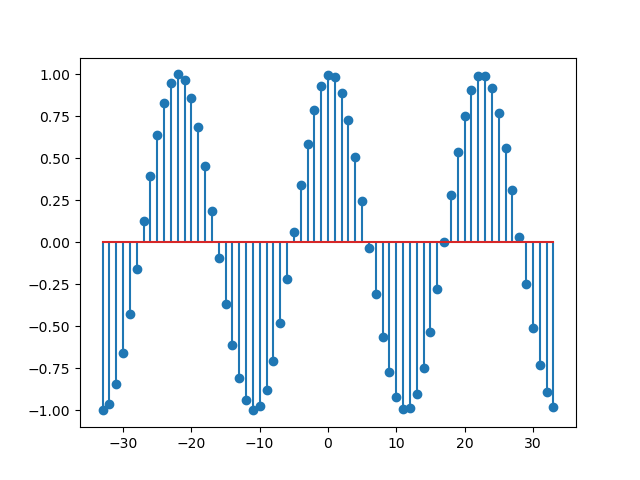
\includegraphics[scale=0.75]{sine_part_b.png}
                        \caption{Output graphic for sine\_part\_b.csv}
                    \end{figure}
                    \begin{figure}[H]
                        \centering
                        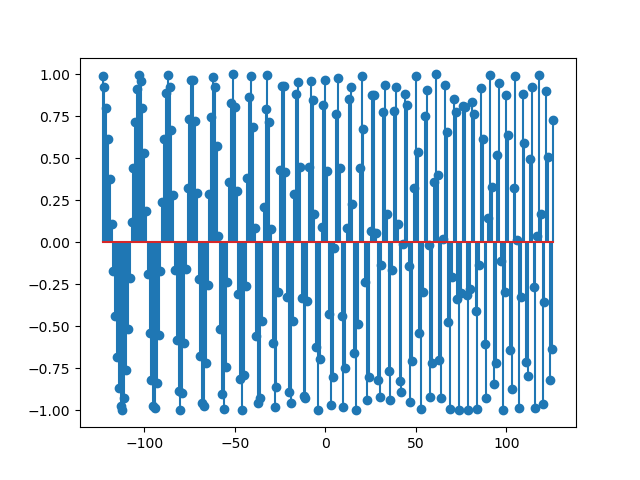
\includegraphics[scale = 0.75]{chirp_part_b.png}
                        \caption{Output graphic for chirp\_part\_b.csv}
                    \end{figure}
                    \begin{figure}[H]
                        \centering
                        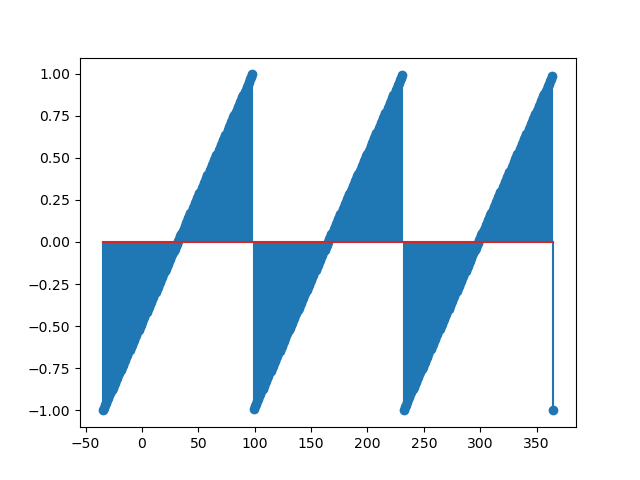
\includegraphics[scale=0.75]{shifted_sawtooth_part_b.png}
                        \caption{Output graphic for shifted\_sawtooth\_part\_b.png}
                    \end{figure}
          \end{enumerate}

\end{enumerate}


\end{document}

